\documentclass[a4paper,12pt,twocolumn]{article}

\usepackage[landscape,top=1cm,bottom=1.4cm,left=1cm,right=1cm,columnsep=1cm]{geometry}
\usepackage[fleqn]{amsmath}
\usepackage{amssymb}
\usepackage{fontspec}
\usepackage{enumitem}
\usepackage{xeCJK}
\usepackage[hidelinks]{hyperref}
\usepackage{tikz}

\setlength{\mathindent}{1.5em}

% Set fonts
\setmainfont{Times New Roman}
\setsansfont{Arial}
\setmonofont{JetBrains Mono}

% Chinese font support
\setCJKmainfont{Iansui}[
  BoldFont=Iansui,
  AutoFakeBold=3.17
]

\pagestyle{plain}
\setlength{\columnseprule}{0.2pt}

\newcommand{\examdate}{2026/05/02}
\newlength{\problemnumberwidth}
\settowidth{\problemnumberwidth}{\textbf{xiii.}\ }
\newcommand{\problemtitle}[2]{%
  \hypertarget{#1}{}%
  \par\vspace{0.4em}%
  \noindent{\large\bfseries #2}\par
  \vspace{0.3em}%
  \hrule
  \vspace{0.9em}%
}
\newcommand{\worksheettoc}{%
  \noindent{\Large\bfseries Contents}\par
  \vspace{0.3em}%
  \hrule
  \vspace{0.9em}%
  \begin{tabular}{@{}p{0.42\columnwidth}p{0.50\columnwidth}@{}}
    \hyperlink{sec:Midterm}{\textbf{Midterm Problems}} &
    \hyperlink{sec:Midterm}{iv, v, vi, vii, x, xi, xiii, 4, 9} \\
  \end{tabular}\par
}
\newcommand{\problem}[2]{%
  \par\noindent
  \hangindent=\problemnumberwidth\relax
  \hangafter=1
  \makebox[\problemnumberwidth][l]{\textbf{#1.}}#2\par
  \vspace{1.4em}%
}
\newcommand{\problemlead}[2]{%
  \par\noindent
  \hangindent=\problemnumberwidth\relax
  \hangafter=1
  \makebox[\problemnumberwidth][l]{\textbf{#1.}}#2\par
}
\newlist{subparts}{enumerate}{1}
\setlist[subparts]{%
  label = (\alph*),
  labelindent=\problemnumberwidth,
  leftmargin=*,
  labelsep=0.5em,
  align=left,
  itemsep=0.2em,
  topsep=0.3em,
  parsep=0pt,
  partopsep=0pt
}
\newlist{romanparts}{enumerate}{1}
\setlist[romanparts]{%
  label = (\roman*),
  labelindent=\problemnumberwidth,
  leftmargin=*,
  labelsep=0.5em,
  align=left,
  itemsep=0.2em,
  topsep=0.3em,
  parsep=0pt,
  partopsep=0pt
}
\newlist{choices}{enumerate}{1}
\setlist[choices]{%
  label = (\Alph*),
  labelindent=\problemnumberwidth,
  leftmargin=*,
  labelsep=0.5em,
  align=left,
  itemsep=0.15em,
  topsep=0.3em,
  parsep=0pt,
  partopsep=0pt
}

\newcommand{\polarregionfigure}{%
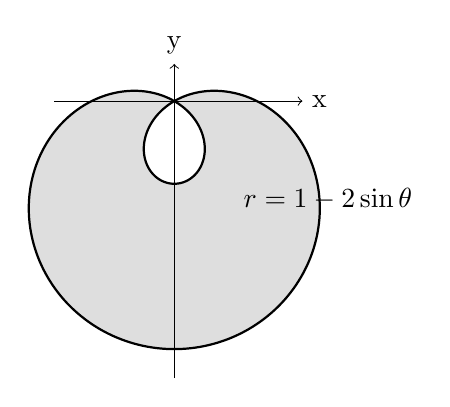
\begin{tikzpicture}[x=1.05cm,y=1.05cm]
  \fill[gray!26]
    plot[domain=150:390, samples=220, variable=\t]
      ({(1 - 2*sin(\t))*cos(\t)}, {(1 - 2*sin(\t))*sin(\t)})
    -- cycle;
  \fill[white]
    plot[domain=30:150, samples=140, variable=\t]
      ({(1 - 2*sin(\t))*cos(\t)}, {(1 - 2*sin(\t))*sin(\t)})
    -- cycle;

  \draw[->, line width=0.35pt] (-1.45,0) -- (1.55,0) node[right] {x};
  \draw[->, line width=0.35pt] (0,-3.35) -- (0,0.45) node[above] {y};

  \draw[black, thick]
    plot[domain=150:390, samples=220, variable=\t]
      ({(1 - 2*sin(\t))*cos(\t)}, {(1 - 2*sin(\t))*sin(\t)});
  \draw[black, thick]
    plot[domain=30:150, samples=140, variable=\t]
      ({(1 - 2*sin(\t))*cos(\t)}, {(1 - 2*sin(\t))*sin(\t)});

  \node[right] at (0.72,-1.18) {$r=1-2\sin\theta$};
\end{tikzpicture}%
}

\begin{document}

\twocolumn[
{\centering
\Large\bfseries Calculus Problems\par
\vspace{0.5em}
\noindent\hfill\normalsize\normalfont\examdate\par
\vspace{0.8em}
}
]

\worksheettoc{}
\vfill\null\newpage

\problemtitle{sec:Midterm}{Midterm Problems}

\problemlead{iv}{The series \(\displaystyle \sum_{n=1}^{\infty}\frac{\cos(n\pi)}{n}\) is}
\begin{choices}
  \item absolutely convergent
  \item conditionally convergent
  \item divergent
\end{choices}
\vspace{1.4em}

\problemlead{v}{The series \(\displaystyle \sum_{n=1}^{\infty}{(-1)}^n\frac{100^n}{n!}\) is}
\begin{choices}
  \item absolutely convergent
  \item conditionally convergent
  \item divergent
\end{choices}
\vspace{1.4em}

\problemlead{vi}{What is the radius of convergence of the series
\(\displaystyle \sum_{n=1}^{\infty}\frac{{(x+1)}^n}{\sqrt{n}\,3^n}\)?}
\begin{choices}
  \item \(0\)
  \item \(\dfrac{1}{3}\)
  \item \(1\)
  \item \(3\)
  \item \(\infty\)
\end{choices}
\vspace{1.4em}

\problemlead{vii}{What is the radius of convergence of the series
\(\displaystyle \sum_{n=0}^{\infty}(2n)!\,x^{2n}\)?}
\begin{choices}
  \item \(0\)
  \item \(1\)
  \item \(2\)
  \item \(3\)
  \item \(\infty\)
\end{choices}
\vspace{1.4em}

\problemlead{x}{Find the sum of \(\displaystyle \sum_{k=1}^{\infty}\frac{1}{k(k+2)}\).}
\begin{choices}
  \item \(\dfrac{1}{4}\)
  \item \(\dfrac{1}{2}\)
  \item \(\dfrac{3}{4}\)
  \item \(\dfrac{5}{2}\)
  \item \(3\)
  \item \(6\)
  \item None of the above
\end{choices}
\vspace{1.4em}

\problemlead{xi}{What is the number of points of intersection of the curves
\(r=\cos 2\theta\) and \(r=\dfrac{1}{2}\)?}
\begin{choices}
  \item \(0\)
  \item \(2\)
  \item \(4\)
  \item \(8\)
  \item None of the above
\end{choices}
\vspace{1.4em}

\problemlead{xiii}{\(\displaystyle \binom{1/2}{4}=\text{?}\)}
\begin{choices}
  \item \(\dfrac{5}{2^4}\)
  \item \(-\dfrac{5}{2^4}\)
  \item \(\dfrac{5}{2^5}\)
  \item \(-\dfrac{5}{2^5}\)
  \item \(\dfrac{5}{2^6}\)
  \item \(-\dfrac{5}{2^6}\)
  \item \(\dfrac{5}{2^7}\)
  \item \(-\dfrac{5}{2^7}\)
\end{choices}
\vspace{1.4em}

\problemlead{4}{Let \(f(x)=\dfrac{1}{{(1-2x^2)}^5}\). Suppose \(f^{(10)}(0)=a\binom{-5}{k}2^n\).}
\begin{romanparts}
  \item \(a=\text{?}\)
  \item \(k=\text{?}\)
  \item \(n=\text{?}\)
\end{romanparts}
\vspace{1.4em}

\problemlead{9}{For the polar curve \(r=1-2\sin\theta\):}
\begin{subparts}
  \item Find \(\dfrac{dy}{dx}\).
  \item Set up the definite integral for the area of the shaded region.
\end{subparts}
\begin{center}
\polarregionfigure{}
\end{center}
\vspace{1.4em}

\end{document}
